% !TEX root = .

\documentclass[a4paper, 12pt, oneside, BCOR1cm,toc=chapterentrywithdots, hidelinks]{scrbook}
\usepackage{scrhack}

\usepackage[a4paper]{geometry}
\usepackage{textcomp}
\usepackage{longtable}
%\usepackage{tabu}

\usepackage[ngerman, english]{babel}
\usepackage[utf8]{inputenc}
\usepackage{graphicx} 
\usepackage{acronym}
\usepackage{url}           	 
\usepackage{hyperref} 	
\usepackage{listings, color}	% for source code
\usepackage{scrlayer-scrpage}	% header and footer line
\usepackage{acronym}
\usepackage[ruled,vlined,algochapter]{algorithm2e}
%\usepackage[nottoc, notlof, notlot]{tocbibind}
\usepackage{blindtext}

\usepackage{chngcntr}
\counterwithout{figure}{chapter}
\counterwithout{table}{chapter}
\counterwithout{algocf}{chapter} 
%\counterwithout{lstlisting}{chapter}
\AtBeginDocument{% the counter is defined later
  \counterwithout{lstlisting}{chapter}%
}
\renewcommand\lstlistingname{Code Fragment}

%for adding comments
\usepackage{verbatim}

% for tables
\usepackage{multirow}
\usepackage[table]{xcolor}
\usepackage{xcolor}

% header and footer line - no header & footer line on pages where a new chapter starts
\pagestyle{scrheadings}
% TU Berlin logo at header
%\chead{
\includegraphics[width=1.2cm]{./img/TU-Berlin-Logo.pdf} 
%}



\begin{document}

\frontmatter
%Titlepage
\thispagestyle{empty}
\begin{center}

\begin{figure}[t]
    \centering
    
\includegraphics[width=3cm]{./img/TU-Berlin-Logo.pdf}%
%    \qquad
%    \includegraphics[width=3.3cm]{dima_logo.png}%
\end{figure}

%\vspace*{0.2cm}
{\LARGE \textbf{Technische Universit\"at Berlin}}

\vspace{0.5cm}

{\large Chair of Database Systems and Information Management\\[1.6mm]}
%{\large Fachgebiet Datenbanksysteme und Informationsmanagement\\[5mm]}

%Fakult\"at IV\\
%Einsteinufer 17\\
%10587 Berlin\\
%https://www.dima.tu-berlin.de\\

\vspace{2.0cm}

{\LARGE Master's Thesis}\\

\vspace{2.45cm}
{\LARGE \textbf{Anonymized Access Control for Distributed Event Stores}}\\
%\vspace*{0.3cm}
%{\LARGE \textbf{second Line}}\\
\vspace{1.0cm}
%{\LARGE Firstname Lastname(s)}
%\vspace*{0.5cm}
Henri Tyl Allgöwer \\
Degree Program: Computer Science\\
Matriculation Number: 454925\\

\vspace*{2.45cm}
\textbf{Reviewers}\\
Prof. Dr. Volker Markl\\
Prof. Dr. Odej Kao\\
\vspace*{0.5cm}
\textbf{Advisor}\\
Rudi Poepsel Lemaitre\\
\vspace{0.5 cm}

\textbf{Submission Date}\\
30.11.2023\\ % 	date of submission
\end{center}


\thispagestyle{empty}
\cleardoublepage
    
%Self-assertion
\newpage

\thispagestyle{empty}

\begin{large}

\vspace*{6cm}

\noindent
Hereby I declare that I wrote this thesis myself with the help of no more than the mentioned literature and auxiliary means.
\vspace{2cm}

\noindent
Berlin, \today

\vspace{3cm}

\hspace*{7cm}%
\dotfill\\
\hspace*{7.5cm}%
\textit{Henri Tyl Allgöwer}

\end{large}
 
\thispagestyle{empty}
\cleardoublepage

% Abstract in Deutsch
\addchap*{Zusammenfassung}
Tipps zum Schreiben dieses Abschnitts finden Sie unter \cite{wallwork_177}

% Abstract
\addchap*{Abstract}
Modern database systems are of incredible importance. Without them, our entire infrastructure would fall apart. Hospitals could no longer properly treat patients, lacking the necessary patient records and treatment history. Banks and financial services would be left unable to execute transactions. Telecommunication services would shut down. These modern database systems often utilize message brokers in combination with stream processing engines. They are capable of accumulating, processing, and distributing data in real-time at an unprecedented rate and volume. With the focus firmly on performance and scalability, data protection has been left behind. A critical oversight as protecting sensitive data is essential in ensuring personal privacy, preventing misuse and fraud, and upholding trust in data handling. At the moment, these database systems provide only very basic access control and lack mechanisms for enforcing privacy policies. Companies often resort to encrypting the data flowing through database systems and focus on external authentification and authorization. Processing encrypted data, however, comes with challenges including computational overhead, added complexity, and performance trade-offs. Decrypting the data again before processing leads back to square one. \par
This thesis introduces a novel model for data anonymization with integrated access control enforcing mechanisms uniquely within modern database systems, more specifically \acfp{DES}. We have realized our model through the development of a new system the \acf{DASH} for Apache Kafka, a leading \ac{DES}. \ac{DASH} is capable of applying a broad variety of anonymization techniques to data streams, uniquely within the database infrastructure. Our tests demonstrate \ac{DASH}'s ability to apply anonymization on individual tuples without introducing performance overhead. We found more complex anonymization techniques, such as those required for achieving k-anonymity on collections of tuples, to be strongly coupled with available system resources. Our evaluation reveals that simpler anonymization techniques are suited for even the highest performance demands, whereas more complex anonymization techniques are more limited in their application.
  
% Acknowledgments  
\addchap*{Acknowledgments}
For recommendations on writing your Acknowledgments see \cite{wallwork_306}.
Thank you to the chair at \ac*{DIMA}

%table of contents
\addtocontents{toc}{\protect\setcounter{tocdepth}{-1}}
\tableofcontents
\addtocontents{toc}{\protect\setcounter{tocdepth}{3}}

%footnote
\newcommand\blfootnote[1]{%
  \begingroup
  \renewcommand\thefootnote{}\footnote{#1}%
  \addtocounter{footnote}{-1}%
  \endgroup
}
\blfootnote{Chapters 3-5 are the core of the thesis, whereas Chapters 1, 2, 6, and 7 provide context. The major contributions should be in Chapters 4 and 5. This structure serves as a guideline and should be customized accordingly. In particular, the generic chapter titles should be replaced with more specific ones, where appropriate (e.g., Chapter 4).} 

%list of figures
\listoffigures

%list of tables
\listoftables



    

    

% List of Abbreviations
\onecolumn
\addchap{List of Abbreviations}
\begin{acronym}[Bash]   
 \acro{DIMA}{Database Systems and Information Management}
\end{acronym}
\onecolumn


%algorithms
\listofalgorithms
\addcontentsline{toc}{chapter}{List of Algorithms}

%In case, code fragments have to be added
%\renewcommand{\lstlistlistingname}{List of Code Fragments}
%\lstlistoflistings
%\addcontentsline{toc}{chapter}{List of Code Fragments}

\mainmatter % comment single chapters for faster compilation
    
    \chapter{Introduction\label{cha:chapter1}}
Distributed event stores capture, store, and process real-time data streams in distributed environments. They have been widely adopted across various sectors, including Fortune 100 companies, governments, healthcare, and transportation industries \cite{kafka} for their efficient, scalable, and fault-tolerant system design. In the modern data-driven world, the growing demand for comprehensive data privacy policies has resulted in increasingly stringent regulations from governments worldwide \cite{GDPR, CCPA}. However, the underlying infrastructure for distributed event stores to adequately support these policies is markedly lacking \cite{Colombo2015}. This disparity poses a unique challenge, particularly when considering the demands of modern database systems to maintain high performance, characterized by low latency and high throughput.\par
The present work aims to examine what techniques can be effectively employed to ensure privacy and security measures, such as access control and data masking, in distributed event stores. Additionally, it aims to explore what strategies can be developed and implemented to ensure that these privacy and security measures have a minimal impact on the performance of distributed event stores. \par
While there exists a body of work focusing on anonymization and data masking for data streaming \cite{Cao2008, KIDS_zhang, anonymizing_IoT}, there is a noticeable gap in research specifically targeting distributed event stores. 
Furthermore, although there are enterprise technologies for managing data flowing into such systems \cite{privitar}, there is limited literature on techniques designed for data already within distributed event stores. Most notably, the concept of integrating \ac{RBAC} within this framework, where the role assigned determines the level of anonymity accorded to the data, is a completely novel approach. \par
The introduction of access control coupled with anonymization in distributed event stores holds the potential to contribute to more advanced, efficient, and secure data handling. By making such tools accessible and cost-effective, companies might be more inclined to prioritize and invest in user data privacy.\par
The overarching goal of this thesis is to design, implement, and evaluate a management framework for distributed event stores. This framework aims to incorporate \ac{RBAC}, granting administrators the capacity to define levels of data anonymization and specify masking functions. By associating levels of anonymization with the number of additional data streams per original data stream, the framework will facilitate nuanced and customizable data privacy measures. Moreover, this plugin will facilitate the assignment of consumers to streams based on their specific roles, further enhancing granular control over data access and privacy within distributed event stores.\par
The scope of this thesis will primarily encompass the exploration of privacy and security measures in the context of distributed event stores. The thesis will delve into the administrative aspects of these technologies, including the implementation and management of access control and data masking functions. Particular attention will be paid to the role of administrators and the impact of their decisions on the performance of these systems. This includes the computational implications of various anonymization techniques. It will involve an in-depth study of different strategies' performance impacts, aiming to minimize overhead while maintaining robust data privacy. At the same time, this thesis will not specifically address or align with any particular data privacy policy such as the \ac{GDPR} \cite{GDPR}. While the thesis is designed around general principles of data privacy and security, it will not provide policy-specific solutions or address the nuances of any specific regulatory framework. Furthermore, the anonymization of data flowing into or out of distributed event stores is beyond the scope of this thesis. The focus will primarily be on the data within the systems, and not on the methods and protocols for handling data entering or leaving these systems. \par
This thesis introduces the \acf{DASH}, a system architected to process data streams into multiple anonymized versions. This design aims to provide users of distributed event stores with a nuanced granularity of anonymization. A comprehensive survey of anonymization techniques is presented, categorizing these methodologies for practical application in various scenarios. \ac{DASH} includes an extensive library of anonymization techniques, offering users the flexibility to tailor the anonymization process to their specific requirements. Additionally, role-based access control is made available as a separate component to assign anonymized versions to streams. This combination of access control with anonymization variety is not only theoretically robust but also practically applicable. Its synergy is highlighted in our theoretical framework chapter, where we showcase a real-world example. Furthermore, this thesis presents a theoretical model designed to simplify future implementations of anonymized access control across various distributed event stores. \par
In the context of this research, we have tested and evaluated \ac{DASH} in an extensive data pipeline environment. We have found \dots \par
The thesis is structured as follows: in Chapter \ref{cha:chapter2} we conduct a literature review. The theoretical framework is constructed in Chapter \ref{cha:chapter3}. Subsequently, Chapter \ref{cha:chapter4} examines in detail the implementation. Tests and their evaluations are addressed in Chapter \ref{cha:chapter5}. Finally, Chapter \ref{cha:chapter6} presents the conclusion and offers an outlook on future work.

    \chapter{Scientific Background\label{cha:chapter2}}
... should include the following:
\begin{itemize}
    \item definitions / technical terms,
    \item theoretical foundations / principles,
    \item descriptions of algorithms, hardware, software, and/or systems employed.
\end{itemize}



\begin{figure}[h]
\centering
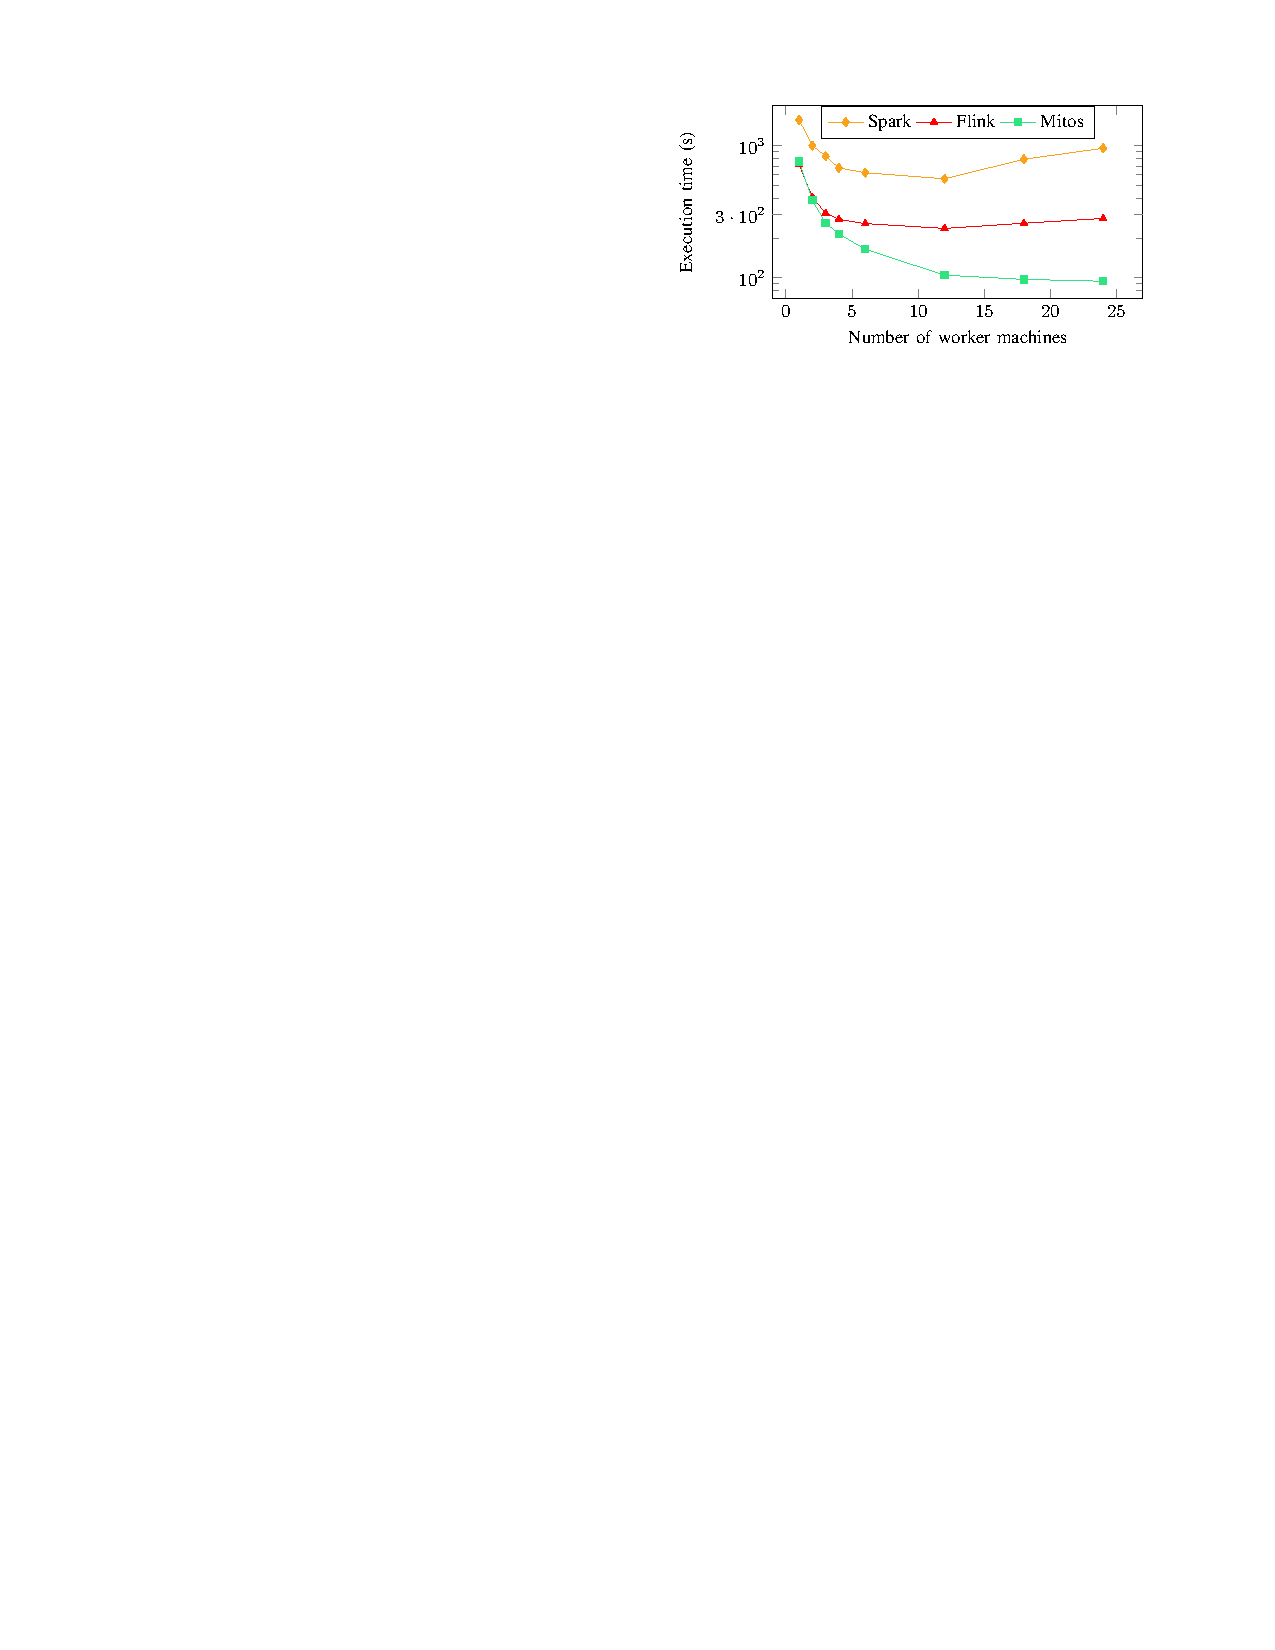
\includegraphics[width=0.6\textwidth]{./img/strong_scaling.pdf}
\caption{Strong scaling for Visit Count\cite{GevayRBMQM21}.}
\end{figure}

% We can leave this out... The advisor can point this out, if it is a concern.
%Suggestion: Figures could be inserted in pdf form to avoid pixelation when the image is magnified.

%This section is intended to give an introduction about relevant terms, technologies and standards in the field of X. You do not have to explain common technologies such as HTML or XML. 



    %\chapter{Implementation \label{sec:metadatatypes}}

\chapter{Research Problem }

... should include the following:
\begin{itemize}

\item a succinct, precise, and unambiguous statement of the research problem or question to be solved,
\item goals and subproblems that will be explored, including the scope of the thesis (i.e., what is in and out of scope).
\end{itemize}
\begin{comment} 
\begin{table}[h!]
\begin{center}
\begin{tabular}{ |c|c|c| } 
 \hline
 Column1 & Column2 & Column3 \\ [0.5ex] 
 \hline
 cell1 & cell2 & cell3 \\ 
 cell4 & cell5 & cell6 \\ 
 cell7 & cell8 & cell9 \\ 
 \hline
\end{tabular}
\caption{An Example Table.}
%\label{table:1}
\end{center}
\end{table}
\end{comment} 


\begin{table}[ht]
\begin{center}
\footnotesize{
\begin{tabular}{ c|c } 
 \hline
  Area (Million sq. miles) & Calling Code \\
  \hline
 0.29 & 56\\
 0.3 & 90\\
 3.8 & 1\\
 0.5 & 51\\
% \rowfont{\color{red}}
\textcolor{red}{600} & \textcolor{red}{9800}\\
 \hline
 \multicolumn{1}{c}{Pearson = 1.0} & \multicolumn{1}{c}{Spearman’s = 0.1}
\end{tabular}
}
\caption{Correlation in the existence of outlier\cite{EsmailoghliQZ21}.}
%\label{table:1}
\end{center}
\end{table}


    \chapter{The Specific Solution Approach }

... should include the following:
\begin{itemize}
\item research methodology (e.g., prototype and experiments, case study, literature survey, theoretical analysis),
\item derivations and descriptions of algorithms, hardware, software, and/or systems developed.
\end{itemize}
\begin{comment} 
\begin{algorithm}
\SetAlgoLined
\KwResult{Write here the result }
 initialization\;
 \While{While condition}{
  instructions\;
  \eIf{condition}{
    instructions1\;
    instructions2\;
    }{
    instructions3\;
    }
    }
 \caption{An Example Algorithm}
 %\label{alg:algorithm1}
\end{algorithm}
\end{comment} 


\begin{algorithm}
\SetAlgoLined
\SetKwInOut{Parameter}{Parameters}
\Parameter{\\e : Tuple to be inserted.\\
te (e) : Event-time of e. }
 S ← slice that covers te (e);\\
  \eIf{S starts at te (e)}{
    //Slice before S must be fixed.\\
    change the type of the slice before S to combined;\\
    add e to S;\\
    }{
    // S does not start at te (e).\\
    change tend (S) to te (e) (excluding te (e) from S);\\
 change type of S to flexible;\\
add slice in [te (e), former tend (S)] with former type of S.\\
add e to the new slice.\\
    }
 \caption{Splitting a Session\cite{TraubGCBKRM20}.}
 %\label{alg:algorithm1}
\end{algorithm}
    \chapter{Experimental (and/or Analytical) Evaluation\label{cha:chapter4}}
\section{Experimental Setup\label{sec:exp}}
... should include the following:
\begin{itemize}

\item define experimental data and workload(s),
\item discussion about the selection and interpretation of the evaluation metrics,
\item discussion about the computing environment, including hardware, software, tools.
\end{itemize}

\begingroup
\renewcommand\thesection{5.X}



\section{Design and an Interpretation of the Results (For each Experiment Class X)}
... should include the following:
\begin{itemize}
\item which experiments will be conducted and why?
\item for each experiment, what are objectives, baselines, and expected results?
\item description and an interpretation of the experimental results,
\item explanation for any anomalies or any unexpected behavior.
\end{itemize}
\endgroup
\begin{comment} 
\section{For each Experiment Class X}

\subsection{Experimental Design}
This sub-section should answer the questions -
\begin{itemize}
\item which experiments will be conducted and why?
\item for each experiment, what are objectives, baselines, and expected results?
\end{itemize}


\subsection{Interpretation of the Results}
This sub-section should include
\begin{itemize}
\item 	description and an interpretation of the experimental results.
\item 	explanation for any anomalies or any unexpected behavior.
\end{itemize}
\end{comment} 


    \chapter{Related Work\label{cha:chapter5}}
... should include the following:
\begin{itemize}

\item state-of-the-art solutions to the problem,
\item related work and a differentiation of your contributions to the related work.

\end{itemize}


%%\lstset{frame=tb,framerule=1pt,keywordstyle=\color{blue}}
%%\begin{comment} 
%%\begin{lstlisting}[ language=SQL,caption= An Example Code Fragment]
%%SELECT 
%%    attribute 
%%FROM 
%%    table
%%WHERE 
%%    attribute = 'value';
%%    
%%\end{lstlisting}
%%\end{comment} 
%%\begin{lstlisting}[ language=Emma,caption= Bounce rate program using nested bags and nested parallel operations\cite{Parallelism}.]
%%val visits: Bag[(Date, IP)] = readFile(...)
%%val visitsPerDay: Bag[(Date, Bag[IP])] = 
%%    visits.groupByKey()
%%visitsPerDay.map{
%%    (day: Date, group: Bag[IP]) =>
%%val countsPerIP = group.map((_, 1)).reduceByKey(_+_)
%%val numBounces = countsPerIP.filter(_._2 == 1).count()
%%val numTotalVisitors = group.distinct().count()
%%val bounceRate =
%%numBounces / numTotalVisitors
%%return bounceRate
%%}

    
%%\end{lstlisting}
    \chapter{Conclusion\label{cha:chapter7}}
In this thesis, we set out to investigate techniques that can be effectively employed to ensure privacy and security measures, such as access control and data masking, in distributed event stores. We evaluated the effectiveness of these techniques by quantifying the performance overhead incurred due to the implementation of additional privacy and security measures. The aim was to bridge the gap in missing underlying infrastructure in distributed event stores to adequately support stringent data privacy regulations by governments worldwide \cite{Colombo2015}. Furthermore, we investigated the intersection of database access control and privacy, an area that has previously been explored by \cite{chaudhuri2011database}. \par
We presented a detailed model incorporating \ac{RBAC} and anonymization techniques in tandem within distributed event stores. We applied this model to Apache Kafka and built the abstraction of \acp{ACL} to \ac{RBAC} as well as the \acf{DASH}. \ac{DASH} is the first system that applies anonymization to data streams in real time for Apache Kafka. By coupling \ac{RBAC} with anonymized access control, our system achieved for the first time anonymization granularity for Apache Kafka. \par
With a comprehensive data pipeline, incorporating Kafka and its administrative component Zookeeper, deployable across various environments via Docker, we tested anonymization techniques and their impact on performance. These tests were performed using a mock dataset hosted on the \ac{DIMA} chair's server. \par
We found that our categorization of anonymization techniques based on the scope of operation translates well to their performance impact. Our experiments showed that value-based anonymization techniques have a negligible impact on performance. Even concatenating multiple anonymization techniques neither negatively impacted latency nor throughput significantly. Similar results were observed for tuple-based 
For attribute-based anonymization techniques, our experiments showed that an upper bound exists for throughput scaling with available resources. Up until that point, no performance decreases were detected, neither in latency nor throughput. Throughput exceeding that threshold, however, suffered significant performance decreases as the time-based windowing technique, that Kafka inherently provides, could not cope with the amount of data per window. A similar observation was made for table-based anonymization techniques. Our implemented k-anonymization was unable to exceed a fixed amount of throughput based on resources. Again for any lower amount of incoming throughput, the performance was not impacted. We attribute this to the computational requirements of the CASTLE algorithms. \par
Independently of the anonymization technique employed, consideration must be given to the additional storage costs. Multiplying data streams necessitates increased storage. \par 
In summary, we showcased a step towards enhancing data privacy in distributed event stores, through the integration of \ac{RBAC} and anonymization techniques creating granular anonymized access control. While acknowledging the challenges and complexities of modern database systems, our work demonstrated a viable pathway for achieving robust data security without compromising performance for masking functions with tuple-at-the-time semantics. As the landscape of data privacy continues to evolve, we believe the insights and methodologies developed during this thesis will contribute to more secure and privacy-conscious data management practices. 

\section{Future Work}
We believe our work creates the foundation of privacy-aware infrastructure within \ac{DES}. From here on out it facilitates the venture into multiple different directions. In the following, we provide some suggestions for potential future work:

\begin{enumerate}
\item \textbf{Graphical User Interface}\\
Adding a graphical user interface for the data officer holds the potential of improving the user experience threefold: First, it would lead to a more fault-tolerant and user-friendly configuration process as it abstracts away the necessity of writing the JSON file by hand. Second, it would simplify the process to no longer require a user with significant technical expertise when the configuration as well as the shell scripts become executable in a UI. This would open up the role of Data Officer to a broader user base. Third, it would truly unify the \ac{RBAC} system with \ac{DASH} as setting up the requirements for the anonymized streams could include the appropriate role-based access control setup. Both would then be achieved simultaneously under the hood.
\item \textbf{Expanding on the Adaptability of DASH}\\
We have developed \ac{DASH} exclusively for Apache Kafka, however, adaptability was always at the back of our mind. It would be interesting to see how \ac{DASH} applies to other Distributed Event Stores, and if our findings for the anonymization techniques translate there as well. As anonymization techniques continue to evolve, it would be intriguing to observe their application to \ac{DASH} and the data streaming realm.
\item \textbf{Parameter Optimization}\\
We found that the choice of parameters had a significant impact on the performance overhead of \ac{DASH}. We believe there is an optimum to be found for a given set of anonymization techniques and data. Taking into consideration information loss, performance overhead, and anonymization robustness, a neural net could be constructed to find the optimal configuration and provide this information to the user.
\end{enumerate}


% ---------------------------------------------------------------

%Bibliography
\begingroup
\raggedright
\bibliographystyle{splncs03}
%\bibliographystyle{acm}
\bibliography{bibliography}
\endgroup

%appendix
\addchap{Appendix A. Further Details on the Solution Approach\label{app:A}}

\begin{sidewaystable}
    \centering
    \tiny
    \begin{longtable}{lllllllllllllll}
        \caption{Extended table of patient data used. The table shows a part of the data used when testing the system. The attribute abbreviations correspond as follows: hgt - height; wgt - weight; ins.\_company - insurance\_company; ins.\_number - insurance\_number, diag. - diagnosis; gluc. - glucose.} \label{tab:patient_data}\\
    \toprule
    \textbf{id} & \textbf{name} & \textbf{address} & \textbf{zip} & \textbf{phone} & \textbf{gender} & \textbf{hgt} & \textbf{wgt} & \textbf{age} & \textbf{ins.\_company} & \textbf{ins.\_number} & \textbf{diag.} & \textbf{gluc.} & \textbf{hba1c} & \textbf{medication} \\
    \midrule
    \endfirsthead
    
    \multicolumn{15}{c}%
    {{\tablename\ \thetable{} -- continued from previous page}} \\
    \toprule
    \textbf{id} & \textbf{name} & \textbf{address} & \textbf{zip} & \textbf{phone} & \textbf{gender} & \textbf{hgt} & \textbf{wgt} & \textbf{age} & \textbf{ins.\_company} & \textbf{ins.\_number} & \textbf{diag.} & \textbf{gluc.} & \textbf{hba1c} & \textbf{medication} \\
    \midrule
    \endhead
    
    \bottomrule
    \endfoot
    
    \bottomrule
    \endlastfoot
    
    
    1 & Sarah Kreusel & Benthinring 6 & 34597 & 0711 98 81331 & Female & 169 & 62 & 95 & 108312586 & L660487647 & E11 & 65 & 9.36 & Metformin \\
    2 & Ronny Kohl & Sauerplatz 42 & 93801 & 089 14407487 & Male & 180 & 73 & 68 & 103508742 & R938242194 & E11 & 157 & 7.77 & Metformin \\
    3 & Lilly Geißler & Mühlestr. 565 & 66369 & 03525914827 & Female & 170 & 51 & 75 & 108928697 & B659387784 & E11 & 98 & 9.79 & Metformin \\
    4 & Marian Bauer & Bruderweg 6/2 & 27618 & 034 56379318 & Male & 189 & 69 & 23 & 103306961 & N988901370 & E10 & 112 & 8.67 & Insulin \\
    5 & Sandra Jähn & Södinggasse 82 & 87339 & 02437 40551 & Female & 166 & 64 & 61 & 101002659 & R453561328 & E10 & 382 & 8.88 & Insulin \\
    6 & Steffen Henk & Junkenallee 03 & 11517 & 03939818024 & Male & 169 & 82 & 57 & 103508742 & Z988986270 & E11 & 96 & 5.76 & Metformin \\
    7 & Dennis Dobes & Trübplatz 465 & 00839 & 08180041538 & Male & 178 & 94 & 86 & 109500490 & T577049432 & E11 & 437 & 7.8 & Metformin \\
    8 & Arif Geisler & Bienstraße 792 & 34510 & 09659 95631 & Diverse & 169 & 61 & 68 & 109500490 & Z210900364 & E10 & 182 & 5.6 & Insulin \\
    9 & Udo Bürger & Kunst Allee 3 & 44149 & 023 1977653 & Male & 182 & 92 & 61 & 109519176 & J339204213 & E11 & 179 & 7.7 & Metformin \\
    10 & Max Mustermann & Wegstr. 42 & 69840 & 0309 049397 & Male & 175 & 80 & 40 & 109500398 & E822232308 & E11 & 120 & 7.0 & Metformin \\
    11 & Erika Mustermann & Hauptstr. 5 & 52820 & 04839768544 & Female & 165 & 65 & 36 & 108817930 & K759451642 & E10 & 140 & 6.8 & Insulin \\
    12 & Julia Schmidt & Bergweg 13 & 33888 & 0612347192 & Female & 168 & 60 & 28 & 109000051 & L858268436 & E11 & 150 & 7.5 & Metformin \\
    13 & Tobias Müller & Seeallee 21 & 78151 & 07899 544559 & Male & 180 & 85 & 55 & 108928697 & I998139981 & E11 & 130 & 6.9 & Metformin \\
    14 & Christina Klein & Talweg 8 & 37111 & 0603328566 & Female & 160 & 55 & 33 & 108888888 & K926100157 & E10 & 135 & 7.2 & Insulin \\
    15 & Uwe Lehmann & Stadtweg 14 & 27417 & 04896 92775 & Male & 175 & 78 & 45 & 109500398 & P619653870 & E10 & 145 & 7.1 & Insulin \\
    16 & Anna Becker & Waldstr. 3 & 10044 & 08645 546756 & Female & 170 & 68 & 31 & 108312586 & D769681473 & E11 & 155 & 7.6 & Metformin \\
    17 & Frank Schubert & Blumenweg 7 & 19364 & 0087010395 & Male & 178 & 82 & 48 & 109500787 & G425120298 & E11 & 125 & 7.4 & Metformin \\
    18 & Kathrin Neumann & Feldstr. 11 & 56066 & 0759017707 & Female & 162 & 58 & 29 & 108814099 & L006897178 & E10 & 138 & 7.3 & Insulin \\
    19 & Lars Hoffmann & Wiesenweg 18 & 75261 & 06671 81305 & Male & 182 & 90 & 52 & 109000051 & A510337443 & E11 & 128 & 6.7 & Metformin \\
    20 & Sabine Fuchs & Bachstr. 22 & 68656 & 06366 46753 & Female & 167 & 63 & 34 & 109500398 & H758511496 & E10 & 132 & 7.0 & Insulin \\
    21 & Dirk Sommer & Forstweg 5 & 73277 & 09304 75332 & Male & 170 & 76 & 43 & 109500787 & M562343754 & E10 & 142 & 6.9 & Insulin \\
    22 & Marie Lange & Hügelstr. 9 & 72773 & 0353876928 & Female & 165 & 61 & 38 & 108313123 & D564564174 & E11 & 160 & 7.8 & Metformin \\
    23 & Oliver Krause & Grabenstr. 2 & 35141 & 01214338986 & Male & 180 & 84 & 50 & 101002659 & U921658735 & E11 & 118 & 6.8 & Metformin \\
    24 & Susanne Winter & Brunnenweg 19 & 01870 & 05033 36428 & Female & 159 & 54 & 32 & 108918320 & Q667879936 & E10 & 137 & 7.1 & Insulin \\
    25 & Markus Winkler & Kanalweg 4 & 90111 & 06309 336421 & Male & 176 & 77 & 46 & 103306961 & X360906143 & E10 & 148 & 7.0 & Insulin \\
    26 & Stefanie Berger & Bahnhofstr. 31 & 83716 & 0371472504 & Female & 169 & 67 & 39 & 108811215 & I955572981 & E11 & 153 & 7.7 & Metformin \\
    27 & Peter Klein & Rosenweg 12 & 30962 & 01556 031663 & Male & 179 & 83 & 51 & 109500398 & H607086736 & E11 & 121 & 6.6 & Metformin \\
    28 & Claudia Schmitt & Kirchweg 29 & 57024 & 09251 652740 & Female & 164 & 59 & 30 & 101575519 & T477237457 & E10 & 136 & 7.2 & Insulin \\
    29 & Heiko Schulz & Sonnenallee 23 & 67294 & 07686863295 & Male & 183 & 88 & 53 & 108928697 & K281348102 & E11 & 127 & 6.5 & Metformin \\
    30 & Birgit Maier & Deichstr. 1 & 28024 & 01098 38370 & Female & 166 & 64 & 35 & 109500044 & G059276367 & E10 & 134 & 6.9 & Insulin \\
    31 & Jan Fischer & Windweg 6 & 60379 & 04196 93544 & Diverse & 171 & 79 & 44 & 109519176 & R260583528 & E10 & 140 & 7.0 & Insulin \\
    32 & Silke Wagner & Steinweg 10 & 09392 & 05613 34703 & Female & 172 & 70 & 37 & 108334056 & O996297939 & E11 & 158 & 7.9 & Metformin \\
    33 & Daniel Meier & Schlossallee 15 & 23078 & 02210254705 & Male & 177 & 81 & 49 & 108817930 & B037958300 & E11 & 124 & 7.5 & Metformin \\
    34 & Heike Schmidt & Lindenweg 20 & 85957 & 01958909813 & Female & 161 & 57 & 27 & 109500398 & V237931864 & E10 & 139 & 7.4 & Insulin \\
    35 & Andreas Schneider & Parkstr. 16 & 67797 & 0118630356 & Male & 184 & 89 & 54 & 103306961 & O573258576 & E11 & 129 & 6.6 & Metformin \\
    36 & Petra Fischer & Mühlenweg 17 & 92660 & 00420619289 & Female & 168 & 62 & 36 & 108918428 & W571231267 & E10 & 131 & 7.1 & Insulin \\
    37 & Christian Weber & Querstr. 8 & 40430 & 0025856617 & Male & 172 & 75 & 42 & 108815718 & M968302874 & E10 & 143 & 6.8 & Insulin \\
    38 & Laura Hoffmann & Auenweg 33 & 45953 & 0778320272 & Female & 173 & 69 & 40 & 108815718 & T881197036 & E11 & 157 & 7.6 & Metformin \\
    39 & Stefan Bauer & Kreuzweg 3 & 24996 & 01188195858 & Male & 178 & 80 & 47 & 108815718 & L541039098 & E11 & 123 & 7.3 & Metformin \\
    \dots & \dots & \dots & \dots & \dots & \dots & \dots & \dots & \dots & \dots & \dots & \dots & \dots & \dots & \dots \\
    n & Henri Allgöwer & Einsteinufer 17 & 10587 & 01765 123456 & Male & 178 & 68 & 27 & 101575519 & T460187489 & E10 & 453 & 10.13 & Insulin \\

    \end{longtable}    
\end{sidewaystable}

\begin{figure}
    \label{table:anonymizers_parameters}
\end{figure}

\begin{figure}
    \label{fig:full_class_diagram}
\end{figure}


\begin{sidewaysfigure}
    \centering
    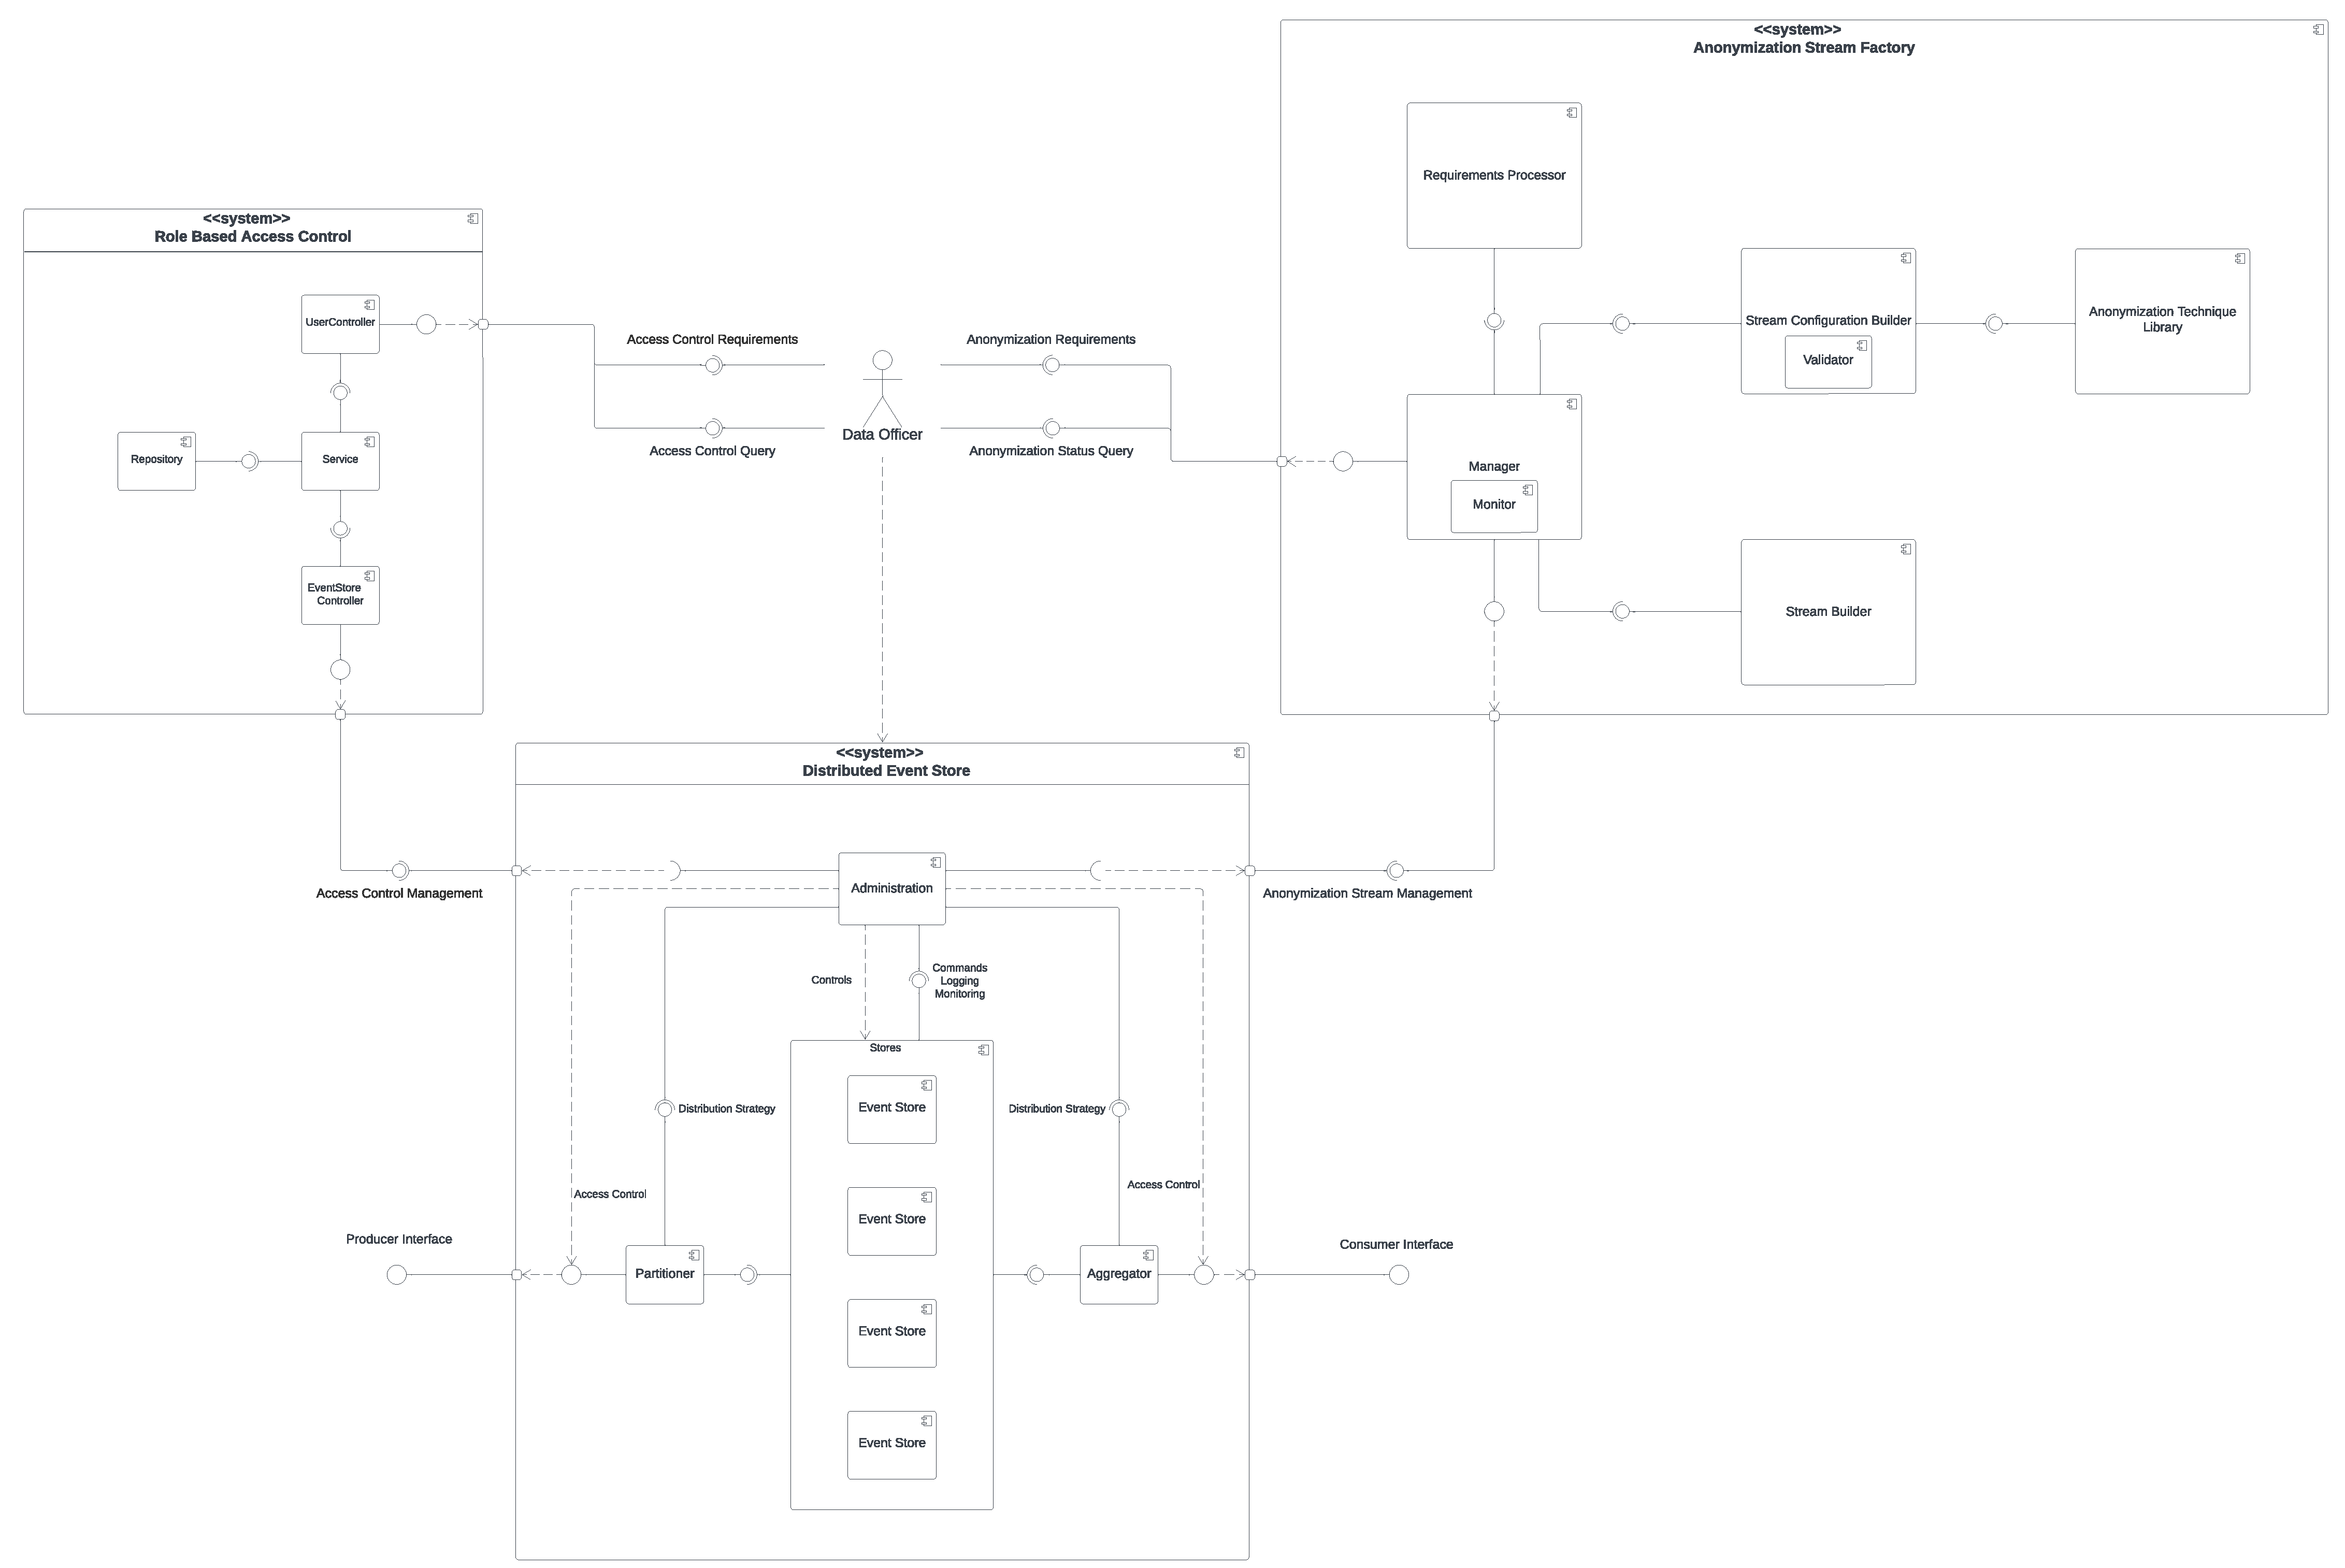
\includegraphics[width=\linewidth]{img/Complete_Component_Diagram.pdf}
    \caption{Full UML Component Diagram for the system as a whole.}
    \label{app:component_diagram}
\end{sidewaysfigure}


\addchap{Appendix B. Extended Version of the Experimental Results}


\end{document}
